\subsection{Définition du besoin}	
	
	La version 1.0 de l’application mobile est réservée à la clientèle \textit{private} (on parle aussi de personnes physiques PP) de NOBC. Cependant, Neuflize ayant la volonté d'étendre la portée de ses services numériques afin de toucher un public toujours plus large, elle a souhaité rendre l'application disponible pour les personnes morales (PM). Ainsi, elle souhaitait inclure très rapidement dans une version 1.1 la clientèle \textit{double relation}, c’est-à-dire la clientèle de type "entreprise" mais qui dispose en même temps dans ses accès des produits "particuliers"; typiquement un entrepreneur qui en plus de ses comptes "entreprises" peut aussi voir/faire de la transaction sur ses comptes "privés". Or, d'un point de vue légal, les entreprises n'ont pas les mêmes droits que les clients private c'est pourquoi des modifications ont dû être apportées aux API. Les méthodes agiles nous apportant une certaine flexibilité, nous avons organisé une réunion avec les métiers afin d'étudier le besoin en détail et déterminer quelles modifications seraient appropriées. \\
	
	A l'issue de cette réunion avec le client, nous avons émis différentes problématiques afin de déterminer les actions à mettre en place au niveau de la couche microservices. Sur le site internet, un abonné double relation dispose d’un bouton lui permettant de visualiser soit ses comptes "entreprises" soit ses comptes "privés". Néanmoins, il n’est pas prévu à ce jour de tel bouton permettant à l’abonné de passer de ses comptes "entreprises" à ses comptes "privés" et inversement sur la version 1.0 de l'application mobile. En effet, celle-ci est réservée à la clientèle "private". De ce fait les produits (comptes, cartes, crédits, titres, etc.) à présenter doivent être des produits "private". De plus, EFS s’est engagé à fournir toutes les informations dans ses API pour que le niveau API microservices puisse faire la distinction entre les comptes et produits "entreprises" et les comptes et produits "privés". Ainsi, le besoin au niveau de la couche API microservices consistait donc à mettre en place des filtres pour présenter/filtrer les données de/vers la couche API de PBI.
	
\subsection{Mise en œuvre}
	
	Avant d'aller plus loin, il est nécessaire de définir ce que sont les \textit{racines}. \hl{TODO : racines} \\
	
	La mise en place de la gestion des doubles relations m'a été confiée et je me suis donc chargé de construire la solution. J'ai d'abord présupposé que les actions menées par EFS avaient été réalisées. Afin de les définir de manière précise, j'ai organisé un point avec une personne métier. Cette dernière a donc pu me les expliciter et elles étaient les suivantes :
	\begin{itemize}
		\item Véhiculer l’information <type de racine> au niveau du back office EFS
		\item Enrichir l’API pour ajouter l’information <type de racine>
		\item Modifier l’API pour remonter les abonnés dont le profil est "particulier" ou "particulier bourse" ainsi que les abonnés dont le profil est "entreprise" ou "entreprise bourse" et qui ont des racines typées "privé" \\
	\end{itemize}
	
	De plus, une table de décision a été mise en place côté EFS (en SQL) dans le but de décider si un type de racine est de type entreprise ou de type particulier afin de le remonter ou non depuis EFS et de préciser l’ordre de présentation (colonne "poids") à exploiter le cas échéant. Cette table était de la forme suivante (les termes métiers importent peu pour la compréhension): \\
	
\begin{table}[h!]
	\center
	\begin{tabular}{| c | c | c |}
     \hline
     Type de racine & Entreprise/Particulier & Poids \\ \hline
     PARF & Particulier & 1\\ \hline
     PARH & Particulier & 2\\ \hline
     STE & Entreprise & 10\\ \hline
     ... & ... & ...\\
     \hline
	\end{tabular}
	\caption{Table de décision pour les doubles relations}
	\label{tableDecisionRacine}
\end{table}
	
	Les règles, issues des spécifications, à respecter concernant l'identification du type des racines étaient les suivantes :
	\begin{itemize}
		\item Si une racine est liée à plusieurs produits dont des comptes :
			\begin{itemize}
				\item Son type entreprise/particulier est porté par la nature du compte
				\item Tous les autres produits (crédit, titre, carte bleue, assurance vie) rattachés à cette racine auront la même nature que le compte
			\end{itemize}
		\item Si une racine est liée à plusieurs produits sans comptes :
			\begin{itemize}
				\item L’API côté EFS devra transmettre l’origine : P (particulier), E (entreprise)
				\item Cette API est cependant susceptible de transmettre <blanc> : alors ce sera le type de la racine qui déterminera si l’ensemble de ses produits est de type particulier ou entreprise
			\end{itemize}
		\item Le cas où une racine est liée à un compte entreprise et un compte particulier n’est pas considéré et est traité comme une anomalie à corriger \\
	\end{itemize}
	
	En outre, un cahier des charges m'a été fourni dans lequel il était stipulé toutes les modifications à effectuer concernant l'appel des services EFS. En effet, comme nous l'avons déjà expliqué, nos services consomment ceux d'EFS afin de la faire de la composition. 
	
	Ainsi, il était par exemple expliqué que le service EFS permettant d'obtenir les assurances vie liées à une racine ne devrait être appelé uniquement pour les clients ne possédant que des produits privés (pas entreprises). 
	
	Pour un autre exemple, EFS expose un service permettant de récupérer les informations de toutes les cartes bleues liées à une racines. Aucun changement n'était demandé concernant l'appel de ce service mais il était nécessaire de filtrer les cartes obtenues afin de ne garder que celles liées à un profil privé et non entreprise. 
	
	Mon objectif était de déterminer quels seraient les microservices impactés et dans quelle mesure par la gestion des doubles relations. Après analyse du cahier fourni, j'ai synthétisé l'ensemble des informations dans le diagramme présent sur la figure \ref{doubleRelation}. \\
	
\begin{figure}[h!]
	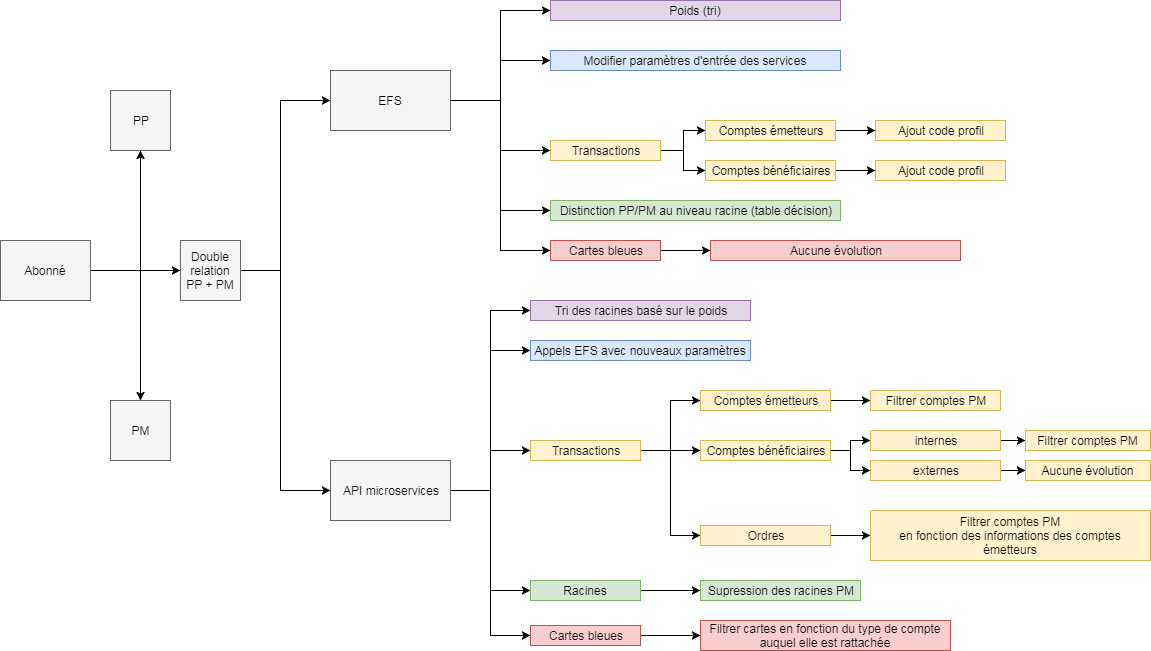
\includegraphics[scale=0.45]{images/travailNeuflizeOBC/doubleRelation/doubleRelation.png}
	\centering
	\caption{Objets impactés par les doubles relations}
	\label{doubleRelation}
\end{figure}

\newpage

	Il était maintenant possible de déterminer les services qui aurraient besoin de développement supplémentaire. D'après ce schéma, les services concernés étaient ceux présent dans le tableau figure \ref{servicesDoubleRelation}. Une fois cela établi il ne restait plus qu'à procéder au développement et à effectuer les modifications nécessaires afin d'assurer la gestion des doubles relations dans la couche API microservices. \\ 
	
\begin{table}[h!]
	\center
	\begin{tabular}{| c | c | c |}
     \hline
     Service & Raison \\ \hline
     accountToDebit & Créer un filtre sur les comptes émetteurs \\ \hline
     addressBook & Créer un filtre sur les comptes bénéficiaires internes \\ \hline
     transactionOverview & Créer un filtre sur les ordres de transaction\\ \hline
     clientList & Créer un filtre sur les racines récupérées \\ & et les trier selon leur poids\\ \hline
     accountOverview & Créer un filtre sur les cartes bleues \\
     Tous & Rajouter le paramètre "codeProfil=PP" dans les appels aux services EFS \\ 
     \hline
	\end{tabular}
	\caption{Modifications par services pour la gestion des doubles relations}
	\label{servicesDoubleRelation}
\end{table}

\subsection{Résultats}

	Comme nous l'avons vu, les modifications à apporter sont mineures et les nouveaux développements sont loin d'être conséquents, mais ces derniers impactent de très nombreux endroits du code et nécessite d'altérer plusieurs services ce qui aurraient pu gêner les autres développeurs dans leur travail. De plus, EFS n'étant pas prêt de son côté, j'ai travaillé en utilisant \textit{WireMock}, un outil permettant de créer des \textit{mocks} qui sont des objets simulés reproduisant le comportement d'objets réels. Ainsi, cela m'a conforté dans l'idée de créer une nouvelle branche sur le github du projet sur laquelle j'ai poussé le code permettant la gestion des doubles relations. Une fois EFS prêt, il sera alors facile de simplement réaliser un merge de cette branche avec la branche master. \\
	
	Bien que la réalisation de cette tâche ne présentait pas de grandes difficultés d'un point de vue de technique, celle-ci m'a permis de me familiariser avec l'aspect relationnel du projet. En effet, nous travaillons en employant des méthodes agiles ce qui m'a conduit a rencontrer le client c'est-à-dire les métiers travaillant dans le même openspace que nous. Ceci m'a permis d'avoir une première expérience complète, bien qu'à petite échelle, allant de la définition du besoin avec le client jusqu'à la réalisation de la fonctionnalité en accompagnant celui-ci tout au long du processus via diverses réunions afin de fixer les points cruciaux. Ensuite, j'ai pu réaliser cette tâche de manière autonome et donc eu la chance de pouvoir mettre en place mes propres solutions tout comme pour la partie concernant les tests fonctionnels, à ceci prêt que dans ce cas il ne s'agissait pas d'un travail indépendant mais en relation direct avec le code source et une livraison, impliquant une certaine confiance.
	En outre, j'ai été contraint d'apporter des modifications à travers toute l'API ce qui m'a permis de pouvoir mieux m'approprier le code et de monter ainsi en compétence sur la stack utilisée et surtout sur le développement de "microservices".